\section{Auswertung}
\label{sec:Auswertung}

\subsection{Winkelrichtgröße}
\label{sec:Winkelrichtgroeße}
Die Winkelrichtgröße wird durch die Formel
\begin{equation}
  D = \frac{F \cdot r}{\phi}
\end{equation}
bestimmt. Die verwendeten Werte sind in Tabelle \ref{tab:winkelrichtgr} angegeben.
\begin{table}
  \centering
  \caption{Messdaten zur Bestimmung der Winkelrichtgröße D}
  \label{tab:winkelrichtgr}
  \begin{tabular}{c c c c}
    \toprule
    $F/N$ & $\phi /^{\circ}$ & $r/m$ & $D/Nm$ \\
    \midrule
    0,1  &  30 & 0,1 & 0,000333 \\
    0,26 &  60 & 0,1 & 0,000433 \\
    0,41 &  90 & 0,1 & 0,000456 \\
    0,56 & 120 & 0,1 & 0,000467 \\
    0,72 & 150 & 0,1 & 0,000480 \\
    0,85 & 180 & 0,1 & 0,000472 \\
    0,48 & 180 & 0,2 & 0,000533 \\
    0,55 & 240 & 0,2 & 0,000458 \\
    0,63 & 270 & 0,2 & 0,000467 \\
    0,69 & 300 & 0,2 & 0,000460 \\
    \bottomrule
  \end{tabular}
\end{table}
\\Sowohl der Mittelwert, als auch die Standardabweichung wurden mit Python bestimmt. Daraus ergibt sich der
gemittelte Wert
\begin{align*}
    D = (0{,}000456 \pm 0{,}000048)\,\mathrm{Nm} .
\end{align*}

\subsection{Eigenträgheitsmoment}
\label{sec:Eigentraegheitsmoment}
Um das Eigenträgheitsmoment der Konstruktion zu bestimmen, messen wir die Schwingunngsdauern unter verschiedenen Abstände $a$ zur Drehachse
der beiden identischen Masse $m_G$ unter dem selben Auslenkungswinkel $\varphi$.
Die beiden Gewichte besitzen die Masse $m_G = 0,2611\, \mathrm{kg}$, die Höhe $h_G = 0,0203\, \mathrm{m}$ und den Radius $R_G = 0,0225\, \mathrm{m}$, mit
den Messunsicherheiten $\Delta m_G = 0,0001\, \mathrm{kg}$ und $\Delta R_G\mathrm{(bzw. h_G)} = 0,0001\, \mathrm{m}$.

\begin{table}
  \centering
  \caption{Messdaten zur Bestimmung des Eigenträgheitsmoment $I_D$}
  \label{tab:eigentrmom}
  \begin{tabular}{c c c c}
    \toprule
    $a/m$ & $T/s^{-1}$ & $a^2/m^2$ & $T^2/s^{-2}$ \\
    \midrule
    0,050 & 2,92 & 0,003 & 8,53 \\
    0,075 & 3,19 & 0,006 & 10,18 \\
    0,100 & 3,92 & 0,010 & 15,37 \\
    0,125 & 4,32 & 0,016 & 18,66 \\
    0,150 & 4,88 & 0,023 & 23,81 \\
    0,175 & 5,58 & 0,031 & 31,14 \\
    0,200 & 5,86 & 0,040 & 34,34 \\
    0,225 & 6,65 & 0,051 & 44,22 \\
    0,250 & 7,14 & 0,063 & 50,98 \\
    0,275 & 7,74 & 0,076 & 59,91 \\
    \bottomrule
  \end{tabular}
\end{table}

Um nun das Eigenträgheitsmoment zu errechnen wird die Tatsache verwendet, dass das Trägheitsmoment der Gewichte bestimmt und
das Gesamtträgheitsmoment ($I_G$ und $I_D$) gemessen werden kann. Es gilt $I_{Ges} = I_D + I_G$. Mithilfe von Formel \ref{eqn:Idiskret} und 8 ergibt sich Folgendes:
\begin{equation}
  \label{eqn:I_ges}
    I_{Ges} = I_D + 2 \cdot \left(\frac{m_G R_G^2}{4} + \frac{m_G h_G^2}{12} \right) + 2 \cdot m_G \cdot a^2
\end{equation}

Die Formel \ref{eqn:I_ges} wird nun in Formel \ref{eqn:I(T)} eingesetzt:

\begin{align*}
  T^2 = 4\pi^2 \cdot \frac{I_D + 2 \cdot \left(\frac{m_G R_G^2}{4} + \frac{m_G h_G^2}{12} \right) + 2 \cdot m_G \cdot a^2}{D}
\end{align*}
\begin{equation}
  \label{eqn:linreg}
  \Leftrightarrow T^2 = \frac{8\pi^2 \cdot m_G}{D}\cdot a^2 + \frac{4\pi^2 \cdot I_D}{D}  + \frac{8\pi^2 \cdot \left(\frac{m_G R_G^2}{4} + \frac{m_G h_G^2}{12} \right)}{D}
\end{equation}
Formel \ref{eqn:linreg} besitzt die Form $y = mx + b$. Wobei 
\begin{equation*}
  y = T^2,\, m = \frac{8\pi^2 \cdot m_G}{D},\, x = a^2 \, \mathrm{und}\, b = \frac{4\pi^2 \cdot I_D}{D}  + \frac{8\pi^2 \cdot \left(\frac{m_G R_G^2}{4} + \frac{m_G h_G^2}{12} \right)}{D}
\end{equation*}
ist. Es wird nun $T^2$ gegen $a^2$ aufgetragen (Abbildung \ref{fig:plot}) und per linearer Regression $m$ und $b$ bestimmt.
 \begin{figure}
   \centering
   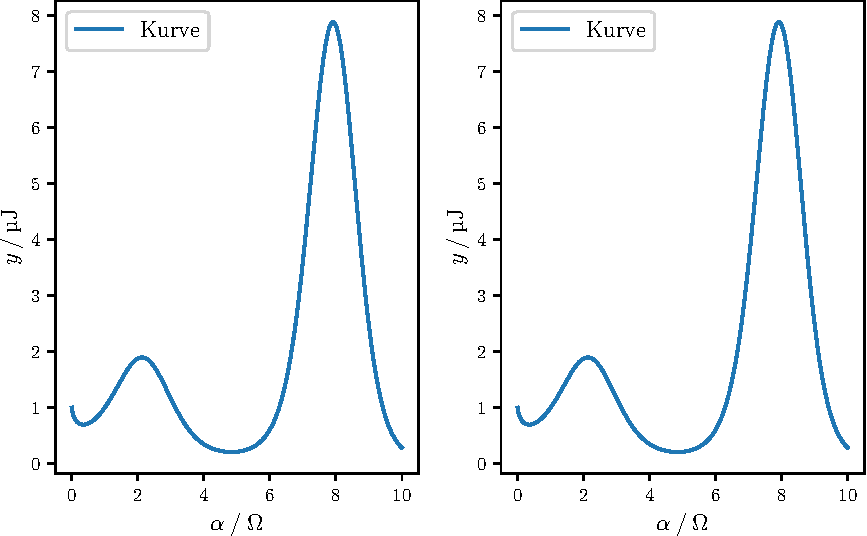
\includegraphics{plot.pdf}
   \caption{Messung des Eigenträgheitsmoments}
   \label{fig:plot}
 \end{figure}
\\
Die lineare Regression wurde mit Python durchgeführt und ergibt für die Gerade $y = mx + b$ die Werte
\begin{align*}
  m = (701{,}1 \pm 15{,}8)\, \frac{1}{\mathrm{s^2 m^2}} \\
  b = (7{,}6 \pm 0{,}6)\, \frac{1}{\mathrm{s^2}} .
\end{align*}
Die Formel für b wird nun nach $I_D$ umgestellt:
\begin{align*}
  b = \frac{4\pi^2 \cdot I_D}{D}  + \frac{8\pi^2 \cdot \left(\frac{m_G R_G^2}{4} + \frac{m_G h_G^2}{12} \right)}{D}
\end{align*}
\begin{align*}
  \Leftrightarrow I_D = \frac{D \cdot b - 8\pi^2 \cdot \left(\frac{m_G R_G^2}{4} + \frac{m_G h_G^2}{12} \right)}{4\pi^2}
\end{align*}
\begin{equation}
  \label{eqn:I_D}
  \Leftrightarrow I_D = \frac{D \cdot b}{4\pi^2} - \left(\frac{m_G R_G^2}{2} + \frac{m_G h_G^2}{6} \right)
\end{equation}

Die Messunsicherheit für $I_D$ wird mithilfe der Gaußschen Fehlerfortpflanzung berechnet (Formel \ref{eqn:Gauss}):

\begin{equation}
  \Delta I_D = 1,2 \cdot 10^{-5} \cdot \mathrm{kg \cdot m^2}
\end{equation}

Also ergibt sich mit Formel \ref{eqn:Gauss} und \ref{eqn:I_D} $I_D$ folgendermaßen:

\begin{equation}
  I_D = \left(0,2 \pm 1,2 \right)\cdot 10^{-5} \mathrm{kg \cdot m^2}
\end{equation}

\subsection{Trägheitsmoment des Zylinders}
\label{sec:TraegheitsmomentdesZylinders}
Der Zylinder hat einen Radius von $R_{Zyl} = 0{,}0494 \, \mathrm{m}$ und eine Höhe von $h_{Zyl} = 0{,}1008 \, \mathrm{m}$
und eine Masse von $m_{Zyl} = 0{,}3678 \, \mathrm{kg}$.
Die Messunsicherheiten der Waage beträgt $\Delta m = 0,0001\, \mathrm{kg}$ und die des Nonius' $\Delta r = 0,0001\, \mathrm{m}$.
\subsubsection{Theoretische Werte}
Das Gesamtträgheitsmoment wird durch Formel \ref{eqn:Izz} bestimmt und der Fehler wird mit der Gaußscheb-Fehlerfortpflanzung (\ref{eqn:Gauss}) bestimmt.
Daraus ergibt sich
\begin{align*}
  I_{Th, Zyl} = \left(4{,}5 \pm 0{,}02 \right) \cdot 10^{-4} \, \mathrm{kg}\cdot\mathrm{m^2}
\end{align*}

\subsubsection{Experimentelle Werte}
Der Zylinder wird auf der Drillachse um den Winkel $\phi_{Zyl} = 90^{\circ}$ ausgelenkt und die Zeit
nach fünf Schwingungen gestoppt.
Durch teilen der Zeitmessungen $Z_{Zyl}$ durch fünf ergeben sich die Schwingungsdauern $T_{Zyl}$. 
Diese sind in Tabelle \ref{tab:T_Zyl} zu finden.
\begin{table}
  \centering
  \caption{Messdaten der Schwingungsdauer des Zylinders}
  \label{tab:T_Zyl}
  \begin{tabular}{c c}
    \toprule
    $Z_{Zyl}/s$ & $T_{Zyl}/s$ \\
    \midrule
    3,94 & 0,79 \\
    3,75 & 0,75 \\
    4,16 & 0,83 \\
    5,78 & 1,16 \\
    3,69 & 0,74 \\
    3,97 & 0,79 \\
    3,85 & 0,77 \\
    3,84 & 0,77 \\
    4,12 & 0,82 \\
    3,88 & 0,78 \\
    \bottomrule
  \end{tabular}
\end{table}
\\
Der Mittelwert und die Abweichung wurden wieder mit Python berechnet.
Aus den Daten ergibt sich
\begin{align*}
  T_{Zyl} = (0{,}82 \pm 0{,}12)\, \mathrm{s} .
\end{align*}
Gaußsche-Fehlerforpflanzung ergibt in Formel \ref{eqn:I(T)}
\begin{align}
  \label{eqn:K_Gauss}
  \Delta I_{K} = \sqrt{\left(\frac{TD}{4\pi^2}\right)^2 \Delta T^2} \nonumber \\
  \Delta I_{K} = \left(\frac{TD}{4\pi^2}\right) \cdot \Delta T.
\end{align}
Aus Formel \ref{eqn:I(T)} und Formel \ref{eqn:K_Gauss} erhält man
\begin{align*}
  I_{Zyl} = (7{,}77 \pm 1{,}14)\cdot 10^{-6}\, \mathrm{mkg^2}.
\end{align*}

\subsection{Trägheitsmoment der Kugel}

Die Kugel hat einen Radius von $R_{Kugel} = 0{,}0726\,\mathrm{m} $ und eine Masse $m_{Kugel} = 1{,}1727 \,\mathrm{kg} $.
Die Messunsicherheiten der Waage beträgt $\Delta m = 0,0001\, \mathrm{kg}$ und die des Nonius' $\Delta r = 0,0001\, \mathrm{m}$.

\label{sec:TraegheitsmomentderKugel}

\subsubsection{Theoretische Werte}

Aus Formel \ref{eqn:Ik} und der Gaußschen-Fehlerfortpflanzung ergibt sich für das Gesamtträgheitsmoment:
\begin{align*}
  I_{Th, K} = \left(24{,}7 \pm 0{,}068 \right) \cdot 10^{-4} \, \mathrm{kg}\cdot\mathrm{m^2}.
\end{align*}

\subsubsection{Experimentelle Werte}
Die Kugel wird auf der Drillachse um $\phi = 90^{\circ}$ ausgelenkt und die Zeit nach drei
Schwingungen gestoppt. Die Schwingungsdauern $T_{Kugel}$ erhält man durch teilen der Zeitmessungen
$Z_{Kugel}$ durch drei. Die Zeitmessungen und berechneten Schwingungsdauern sind in
Tabelle \ref{tab:T_Kugel} zu finden.
\begin{table}
  \centering
  \caption{Messdaten der Schwingungsdauer der Kugel}
  \label{tab:T_Kugel}
  \begin{tabular}{c c}
    \toprule
    $Z_{Kugel}/s$ & $T_{Kugel}/s$ \\
    \midrule
    5,94 & 1,98 \\
    5,71 & 1,90 \\
    5,62 & 1,87 \\
    5,47 & 1,82 \\
    5,63 & 1,88 \\
    5,47 & 1,82 \\
    5,75 & 1,92 \\
    5,47 & 1,82 \\
    5,66 & 1,89 \\
    5,57 & 1,86 \\
    \bottomrule
  \end{tabular}
\end{table}
\\
Der Mittelwert und die Abweichug wurden mit Hilfe von Python bestimmt. Aus den Werten erhält man
\begin{equation}
  T_{Kugel} = (1{,}88 \pm 0{,}05)\, \mathrm{s} .
\end{equation}
Aus Formel \ref{eqn:I(T)} und Formel \ref{eqn:K_Gauss} erhält man
\begin{align*}
  I_{Kugel} = (4{,}08 \pm 0{,}11)\cdot 10^{-6}\, \mathrm{mkg^2}.
\end{align*}

\subsection{Maße des Körpers}
\label{sec:maskoerper}
Der Körper wird durch sechs Zylinder angenähert. Er besteht aus einem Oberkörper, einem Kopf und jeweils zwei Armen und Beinen.
Die Abmessungen lassen sich in Tabelle \ref{tab:r_Koerper} finden. Außerdem hat der Körper eine Masse von $m_{Puppe} = 0{,}1683\,\mathrm{kg}$
\begin{table}
  \centering
  \caption{Maße des Körpers}
  \label{tab:r_Koerper}
  \begin{tabular}{c c c c}
    \toprule
    $r_{Oberk\ddot{o}rper}/m$ & $r_{Beine}/m$ & $r_{Arme}/m$ & $r_{Kopf}/m$ \\
    \midrule
    0,0203 &  0,0091 &  0,0063 & 0,0109 \\
    0,0160 &  0,0084 &  0,0071 & 0,0145 \\
    0,0199 &  0,0084 &  0,0066 & 0,0117 \\
    0,0104 &  0,0065 &  0,0073 & 0,0110 \\
    0,0194 &         &         &        \\
    0,0167 &         &         &        \\
    \bottomrule
  \end{tabular}
\end{table}
Die Standardabweichung und die Mittelwerte wurden mit Python berechnet.
\begin{align*}
  R_{Oberk\ddot{o}rper}       = (0{,}0171 \pm 0{,}0034)\, \mathrm{m} \\
  R_{Beine}      = (0{,}0081 \pm 0{,}0010)\, \mathrm{m} \\
  R_{Arme}       = (0{,}0068 \pm 0{,}0004)\, \mathrm{m} \\
  R_{Kopf}       = (0{,}0120 \pm 0{,}0015)\, \mathrm{m} \\
\end{align*}
Die gemessen Höhen der Zylinder sind als
\begin{align*}
  h_{Oberk\ddot{o}rper}       = (0{,}0991 \pm 0{,}0001)\, \mathrm{m} \\
  h_{Beine}      = (0{,}1502 \pm 0{,}0001)\, \mathrm{m} \\
  h_{Arme}       = (0{,}1129 \pm 0{,}0001)\, \mathrm{m} \\
  h_{Kopf}       = (0{,}0519 \pm 0{,}0001)\, \mathrm{m} \\
\end{align*}
angegeben.

Es wird die Massendichte bestimmt, um die Massen und somit die Trägheitsmomente auszurechnen:

\begin{align*}
& \rho = \frac{M_{Ges}}{V_{Ges}} \\
&  V_{Ges} = V_{Oberk\ddot{o}rper} + V_{Kopf} + 2 \cdot V_{Arme} + 2 \cdot V_{Beine} \\
&  = \pi \cdot \left(R_{Oberk\ddot{o}rper}^2  \cdot h_{Oberk\ddot{o}rper} + R_{Kopf}^2 \cdot h_{Kopf} + 2 \cdot R_{Arme}^2 \cdot h_{Arme} +2 \cdot R_{Beine}^2 \cdot h_{Beine} \right) \\
&  = (2{,}09 \pm 0{,}38) \cdot 10^{-4} \, \mathrm{m^3} \\
& \rho = (805{,}263 \pm 146{,}412) \, \mathrm{\frac{kg}{m^3}}
\end{align*}

Daraus lässt sich nun die Masse der einzelnen Zylinder berechnen:

\begin{align*}
  &  m_Zyl = \rho \cdot V_Zyl \\
  &  m_{Oberk\ddot{o}rper} = \rho \cdot \pi R_{Ober\ddot{o}rper}^2 h_{Ober\ddot{o}rper} = 0{,}073308 \pm 0{,}032055 \mathrm{kg} \\
  &  m_{Beine} = \rho \cdot \pi R_{Beine}^2 h_{Beine} = 0{,}02493 \pm 0{,}007644 \, \mathrm{kg} \\
  &  m_{Arme} = \rho \cdot \pi R_{Arme}^2 h_{Arme} = 0{,}013207 \pm 0{,}00286 \, \mathrm{kg} \\
  &  m_{Kopf} = \rho \cdot \pi R_{Kopf}^2 h_{Kopf} = 0{,}018907 \pm 0{,}00609 \, \mathrm{kg} \\
\end{align*}

\subsection{Trägheitsmoment der Puppe in Körperhaltung 1}
\label{sec:TraegheitsmomentderPuppeinKoerperhaltung 1}
\subsubsection{Theoretische Werte}

Um das Gesamtträgheitsmoment zu errechnen, werden die Einzelträgheitsmomente der Zylinder berechnet:

Für den Oberkörper gilt, dass die Drehachse durch seinen Schwerpunkt verläuft. Wir können somit Formel \ref{eqn:Izz} anwenden ohne den 
Satz von Steiner zu verwenden (Formel \ref{eqn:Steiner}):
\begin{align*}
  & I_{Oberk\ddot{o}rper} = \frac{m_{Oberk\ddot{o}rper}R_{Oberk\ddot{o}rper}^2}{2} = (1{,}0718 \pm 0{,}6335) \cdot 10^{-5} \, \mathrm{\frac{kg}{m^3}}
\end{align*}

Für den Kopf gilt das Gleiche, wie für den Oberkörper:

\begin{align*}
  & I_{Kopf} = \frac{m_{Kopf}R_{Kopf}^2}{2} = (0{,}1361 \pm 0{,}0555) \cdot 10^{-5} \, \mathrm{\frac{kg}{m^3}}
\end{align*}

In Position 1 hängen die Arme an den Seiten des Oberkörpers herunter, das heißt die Drehachse ist um $a = R_{Oberk\ddot{o}rper} + R_{Arme} = 0{,}0239 \pm 0{,}003716 \, \mathrm{m}$
verschoben und wir müssen die Formeln \ref{eqn:Steiner} und \ref{eqn:Izz} anwenden:

\begin{align*}
  & I_{Arme,1} = \frac{m_{Arme}R_{Arme}^2}{2} = (0{,}0305 \pm 0{,}0075) \cdot 10^{-5} \, \mathrm{\frac{kg}{m^3}} \\
  & I_{Arme,2} = I_{Arme,1} + m_{Arme} \cdot a^2 = (0{,}7849 \pm 6{,}8889) \cdot 10^{-5} \, \mathrm{\frac{kg}{m^3}}
\end{align*}

Bei den Beinen gilt ähnliches, nur dass diese um $a = h_{Beine} \cdot 0{,}5 = 0{,}01247 \pm 0{,}00382 \, \mathrm{m}$ verschoben sind
und wir die Formeln \label{eqn:Izx} und \ref{eqn:Steiner} verwenden:

\begin{align*}
  & I_{Beine,1} = \frac{m_{Beine}R_{Beine}^2}{4} + \frac{m_{Beine}h_{Beine}^2}{12} =  \\
  & I_{Beine,2} = I_{Beine,1} + m_{Beine} \cdot a^2 = 
\end{align*}

\subsubsection{Experimentelle Werte}
Die Puppe wird in der ersten Körperhaltung um $\phi = 90^{\circ}$ ausgelenkt und die Zeit $Z_{K1}$ nach drei
Schwingungen gemessen. Die Schwingungsdauern $T_{K1}$ erhält man durch teilen der Zeitmessung durch drei. Die Zeitmessungen und
Schwingunsdauern sind in Tabelle \ref{tab:Koerper1} angegeben.
\begin{table}
  \centering
  \caption{Messdaten der Schwingunsdauer des Körpers in der ersten Position}
  \label{tab:Koerper1}
  \begin{tabular}{c c}
    \toprule
    $Z_{K1}/s$ & $T_{K1}/s$ \\
    \midrule
    2,75 & 0,92 \\
    2,66 & 0,89 \\
    2,66 & 0,89 \\
    2,90 & 0,97 \\
    3,16 & 1,05 \\
    2,56 & 0,85 \\
    2,47 & 0,82 \\
    2,75 & 0,92 \\
    2,53 & 0,84 \\
    2,78 & 0,93 \\
    \bottomrule
  \end{tabular}
\end{table}
\\
Mit Hilfe von Python lässt sich der Mittelwert und die Abweichung bestimmen. Aus den Messdaten
erhält man
\begin{align*}
  T_{K1} = (0{,}91 \pm 0{,}06)\, \mathrm{s} .
\end{align*}
Mit Hilfe von Formel \ref{eqn:I(T)} und Formel \ref{eqn:K_Gauss} lässt sich das Trägheitsmoment bestimmen als
\begin{align*}
  I_{K1} = (9{,}57 \pm 0{,}63) \cdot 10^{-6}\, \mathrm{mkg^2}.
\end{align*}

\subsection{Trägheitsmoment der Puppe in Körperhaltung 2}
\label{TraegheitsmomentderPuppeinKoerperhaltung2}
\subsubsection{Theoretische Werte}

\subsubsection{Experimentelle Werte}
Die Puppe wurde in der zweiten Körperhaltung um $\phi = 90^{\circ}$ ausgelenkt und die Zeit $Z_{K2}$
wurde nach drei Schwingungen gestoppt. Die Schwingungsdauer $T_{K2}$ wird durch teilen von $Z_{K2}$
durch drei berechnet. Die Zeitmessungen und Schwingungdsdauern sind in Tabelle \ref{tab:Koerper2} zu finden.
\begin{table}
  \centering
  \caption{Messdaten der Schwingugnsdauer des Körpers in der zweiten Position}
  \label{tab:Koerper2}
  \begin{tabular}{c c}
    \toprule
    $Z_{K2}/s$ & $T_{K2}/s$ \\
    \midrule
    1,91 & 0,64 \\
    1,75 & 0,58 \\
    1,75 & 0,58 \\
    1,84 & 0,61 \\
    1,68 & 0,56 \\
    1,84 & 0,61 \\
    1,81 & 0,60 \\
    1,66 & 0,55 \\
    1,84 & 0,61 \\
    1,81 & 0,60 \\
    \bottomrule
  \end{tabular}
\end{table}
\\
Sowohl der Mittelwert, als auch die Standarabweichung wurde mit Python bestimmt.
\begin{align*}
  T_{K2} = (0{,}59 \pm 0{,}03)\, \mathrm{s} .
\end{align*}
Mit Hilfe von Formel \ref{eqn:I(T)} und Formel \ref{eqn:K_Gauss} lässt sich das Trägheitsmoment bestimmen als
\begin{align*}
  I_{K2} = (4{,}02 \pm 0{,}20) \cdot 10^{-6}\, \mathrm{mkg^2}.
\end{align*}
